\chapter{Конструкторский раздел}

\section{Трудоемкость алгоритмов}\label{estimate}
Для получения функции трудоемкости алгоритма необходимо ввести модель оценки трудоемкости. Трудоемкость "элементарных" операций оценивается следующим образом:
\begin{enumerate}
	\item Трудоемкость 1 имеют операции:
	\begin{equation*}\label{math:simple}
		\begin{array}{cc}
			+, -, =, <, >, <=, >=, ==, +=, -=,\\
			++, --, [], \&\&, ||, >>, << \\
		\end{array}
	\end{equation*}
	\item Трудоемкость 2 имеют операции:
	\begin{equation*}\label{math:complex}
		*, /, \char`\\ , \%
	\end{equation*}	
	\item Трудоемкость конструкции ветвления определяется согласно формуле \ref{math:if}
	\begin{equation}\label{math:if}
		f_{if} = f_{condition} + 
		\begin{sqcases}
			min\left(f_{true} , f_{false}\right) \text{ в лучшем случае,} \\
			max\left(f_{true} , f_{false}\right) \text{ в худшем случае.} \\
		\end{sqcases}
	\end{equation}
	\item Трудоемкость цикла расчитывается по формуле \ref{math:loop}
	\begin{equation}\label{math:loop}
		f_{loop} = f_{init} + f_{cmp} + N \left(f_{body} + f_{inc} + f_{cmp}\right),
	\end{equation}
	\begin{equation*}
		\begin{array}{lllll}
			\text{где} \\
			f_{init} - \text{трудоемкость инициализации,} \\
			f_{body} - \text{трудоемкость тела цикла,} \\
			f_{iter} - \text{трудоемкость инкремента,} \\
			f_{cmp} - \text{трудоемкость сравнения,} \\
			N - \text{количество повторов.}
		\end{array}
	\end{equation*}
	\item Трудоемкость вызова функции равна 0.
\end{enumerate}

\section{Оптимизация алгоритма Копперсмита -- Винограда}\label{sect:optimize}
Алгоритм Копперсмита -- Винограда можно оптимизировать следующим образом:
\begin{itemize}
	\item Счетчики цикла можно объявить единожды и обнулять их по требованию. В этом случае стоимость инициализации при расчете трудоемкости цикла сократится;
	\item Увеличение числа на определенное число можно заменить на операцию $+=$, поскольку она имеет меньший вес чем в сумме сложение и присвоение;
	\item Для алгоритма худшим случаем являются матрицы с нечётным общим размером, а лучшим - с четным. Соответственно, алгоритм можно ускорить в соответствии с четностью размера.
\end{itemize}

\section{Трудоемкость алгоритмов}

\subsection{Классический алгоритм}

Пусть на вход алгоритму поступают матрицы $M_{left}$ и $M_{right}$ с размерностью $n \times m$ и $m \times q$. Тогда трудоемкость классического алгоритма определяется по формуле \ref{math:alg}
\begin{multline}\label{math:alg}
	f_{alg} = f_{loop_i} = 2 + n\left(2 + f_{loop_j}\right) = 2 + n\left(2 + 2 + q\left(2 + f_{loop_k}\right)\right) = \\
	= 2 + n\left(2 + 2 + q\left(2 + 2 + 12 \cdot m\right)\right) \approx 10mnq = 10MNK
\end{multline}
\subsection{Алгоритм Копперсмита -- Винограда}\label{win-estimate}
Пусть на вход алгоритму поступают матрицы $M_{left}$ и $M_{right}$ с размерностью $n \times m$ и $m \times q$. Тогда трудоемкость алгоритма Копперсмита -- Винограда расчитывается как \ref{math:cw-cost}:
\begin{equation}\label{math:cw-cost}
	f_{CW} = f_{init} + f_{precomp} + f_{fill} + f_{even},
\end{equation}
где:
\begin{itemize}
	\item $f_{init}$ -- инициализация массивов для препроцессирования, стоимость которой равна \ref{math:cw-init}
	\begin{equation}\label{math:cw-init}
		f_{init} = n + q
	\end{equation} 
	\item $f_{precomp}$ -- трудоемкость заполнения массивов , которая вычисляется по формуле \ref{math:cw-precomp}:
		\begin{equation}\label{math:cw-precomp}
		f_{precomp} = f_{rows} + f_{cols},
	\end{equation} 
	где:
	\begin{itemize}
		\item $f_{rows}$ -- трудоемкость заполнения массива строк, состоящая из двух циклов, трудоемкость которых, согласно модели вычисления в разделе \ref{math:loop} равна \ref{math:cw-precomp-rows}:
		 \begin{equation}\label{math:cw-precomp-rows}
		 	f_{rows} = 2 + n\left(8m - 6\right)
		 \end{equation}
		\item $f_{cols}$ -- трудоемкость заполнения массива столбцов, состоящая из двух циклов, трудоемкость которых, согласно модели вычисления в разделе \ref{math:loop} равна \ref{math:cw-precomp-cols}
		\begin{equation}\label{math:cw-precomp-cols}
			f_{cols} = 2 + q\left(8m - 6\right)
		\end{equation}
	\end{itemize}
	\item $f_{fill}$ -- цикл заполнения матрицы, трудоемкость которого, согласно модели вычисления в разделе \ref{math:loop} равна \ref{math:cw-fill}:
	\begin{equation}\label{math:cw-fill}
		f_{fill} = 2 + n\left(2 + q\left(2 + 21\dfrac{m - 1}{2}\right)\right)
	\end{equation}
	\item $f_{even}$ -- цикл для дополнения умножения в случае нечетной размерности, который, согласно модели вычисления в разделе \ref{math:loop} равна \ref{math:cw-even}:
	\begin{equation}\label{math:cw-even}
		f_{fill} = 
		\begin{sqcases}
			2 & \text{л. с,} \\ 
			2 + n\left(2 + 14q\right) & \text{х. с.}
		\end{sqcases}
	\end{equation}
\end{itemize}
Значит, трудоемкость алгоритма Копперсмита -- Винограда в лучшем случае равна \ref{math:cw-numeric-best}:

\begin{multline}\label{math:cw-numeric-best}
	f_{CW} = n + q + 2 + n\left(8m - 6\right) + 2 + q\left(8m - 6\right) + \\
	+ 2 + n\left(2 + q\left(2 + 21\dfrac{m - 1}{2}\right)\right) +\\
	+ 2 \approx \dfrac{21}{2}mnq = 10.5MNK
\end{multline}

В худшем случае соответственно \ref{math:cw-numeric-worst}:

\begin{multline}\label{math:cw-numeric-worst}
	f_{CW} = n + q + 2 + n\left(8m - 6\right) + 2 + q\left(8m - 6\right) + \\
	+ 2 + n\left(2 + q\left(2 + 21\dfrac{m - 1}{2}\right)\right) +\\
	+ 2 + n\left(2 + 14q\right) \approx \dfrac{21}{2}mnq = 10.5MNK
\end{multline}


\subsection{Оптимизация алгоритма Копперсмита -- Винограда}\label{o-win-estimate}

Пусть на вход алгоритму поступают матрицы $M_{left}$ и $M_{right}$ с размерностью $n \times m$ и $m \times q$. Тогда трудоемкость оптимизированного алгоритма Копперсмита -- Винограда расчитывается как \ref{math:cw-o-cost}:
\begin{equation}\label{math:cw-o-cost}
	f_{CW} = f_{init} + f_{precomp} + f_{fill} % + f_{even},
\end{equation}
Здесь $f_{init}$ расчитывается по формуле \ref{math:cw-init}. Однако, отличаться будет стоимость $f_{precomp}$ благодаря замене присваивания и сложения на оператор $+=$ и предварительной инициализации индексов. Соответственно, $f_{precomp}$ удовлетворяет формуле\ref{math:cw-o-precomp}:
\begin{equation}\label{math:cw-o-precomp}
	f_{precomp} = f_{rows} + f_{cols} = 2 + n\left(9 \dfrac{m - 1}{2}\right) + q\left(9 \frac{m - 1}{2}\right)
\end{equation}
Трудоемкость цикла заполнения матрицы расчитывается следующим образом (\ref{math:cw-o-fill}):
\begin{equation}\label{math:cw-o-fill}
	f_{fill} = 
	\begin{sqcases}
		1 + n \left(2 + q\left(2 + 17\dfrac{m - 1}{2}\right)\right) & \text{л. с,} \\[2.2ex]
		1 + n \left(2 + q\left(9 + 17\dfrac{m - 1}{2}\right)\right) & \text{х. с.}
	\end{sqcases}
\end{equation}

Значит, трудоемкость алгоритма Копперсмита -- Винограда в лучшем случае равна \ref{math:cw-o-numeric-best}:

\begin{multline}\label{math:cw-o-numeric-best}
	f_{CW} = n + q + 2 + n\left(9 \dfrac{m - 1}{2}\right) + q\left(9 \frac{m - 1}{2}\right) + 1 + \\
	n \left(2 + q\left(2 + 17\dfrac{m - 1}{2}\right)\right)  \approx \dfrac{17}{2}mnq = 9.5MNK 
\end{multline}

В худшем случае соответственно \ref{math:cw-o-numeric-worst}:

\begin{multline}\label{math:cw-o-numeric-worst}
	f_{CW} = n + q + 2 + n\left(9 \dfrac{m - 1}{2}\right) + q\left(9 \frac{m - 1}{2}\right) + 1 + \\
	n \left(2 + q\left(9 + 17\dfrac{m - 1}{2}\right)\right) \approx \dfrac{17}{2}mnq = 9.5MNK 
\end{multline}

\section{Схемы алгоритмов}
На рисунке \ref{fig:alg} приведена схема классического алгоритма умножения матриц. На рисунках \ref{fig:win-1}, \ref{fig:win-2}, \ref{fig:win-3} приведена схема алгоритма Копперсмита -- Винограда, на рисунках  \ref{fig:prep-r}, \ref{fig:prep-c} приведена схема алгоритмов препроцессирования. Рисунки  
\ref{fig:win-o-1}, \ref{fig:win-o-2} демонстрируют схему оптимизированного алгоритма Копперсмита -- Винограда.\newpage

\begin{figure}[H]
	\centering
	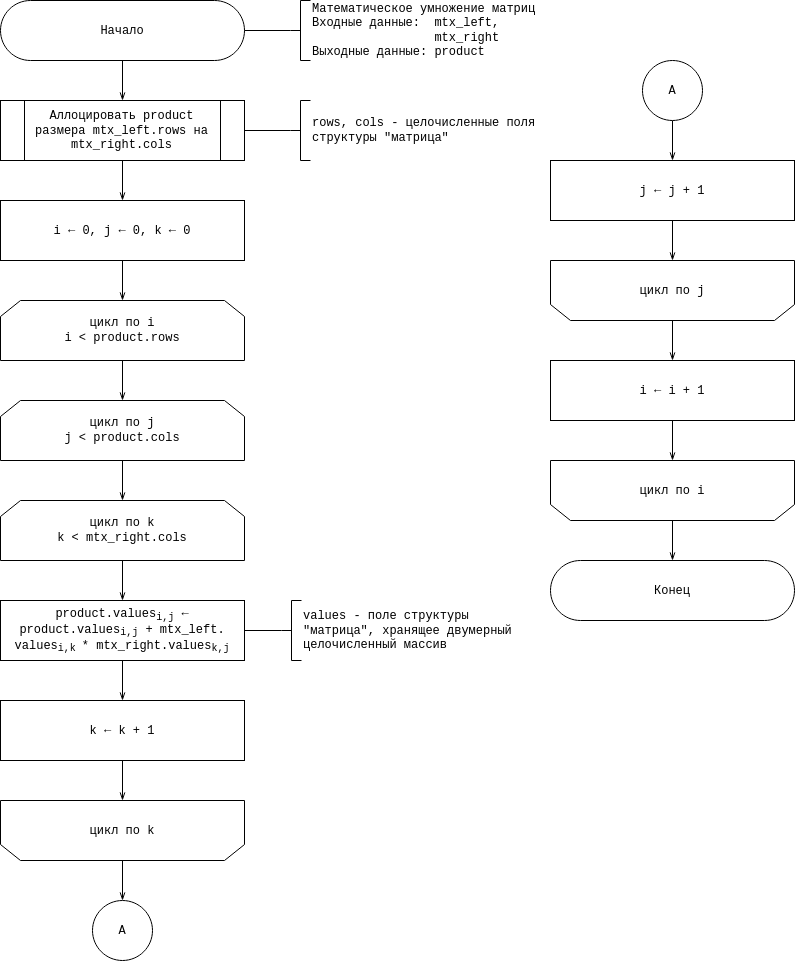
\includegraphics[width=\linewidth]{assets/mtx-alg.drawio.png}
	\caption{Схема классического алгоритма умножения матриц}
	\label{fig:alg}
\end{figure}

\begin{figure}[H]
	\centering
	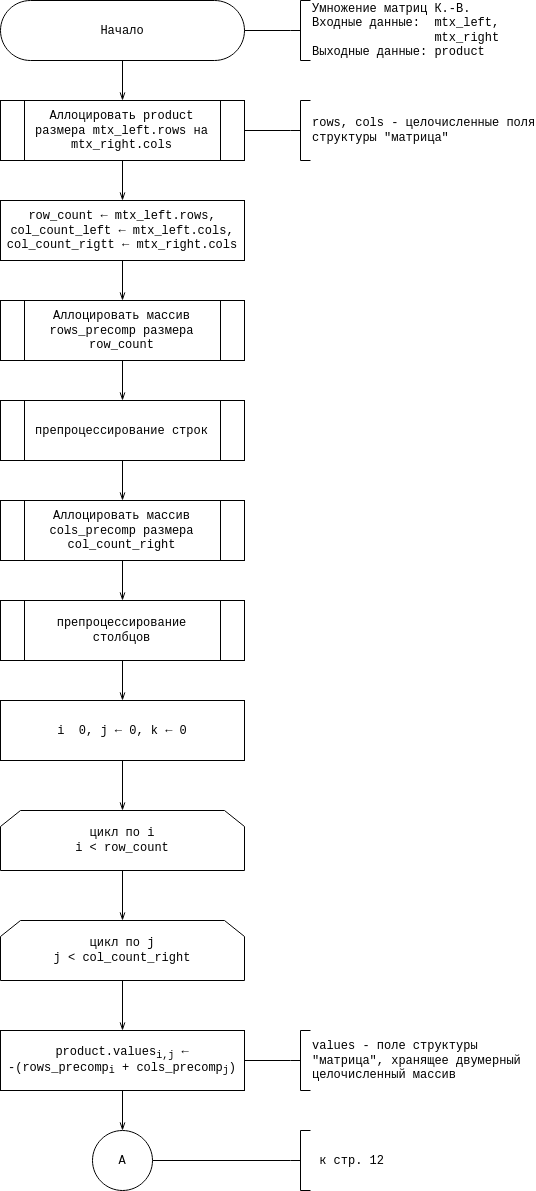
\includegraphics[width=0.65\linewidth]{assets/mtx-win1.drawio.png}
	\caption{Схема алгоритма умножения матриц Копперсмита -- Винограда (начало)}
	\label{fig:win-1}
\end{figure}

\begin{figure}[H]
	\centering
	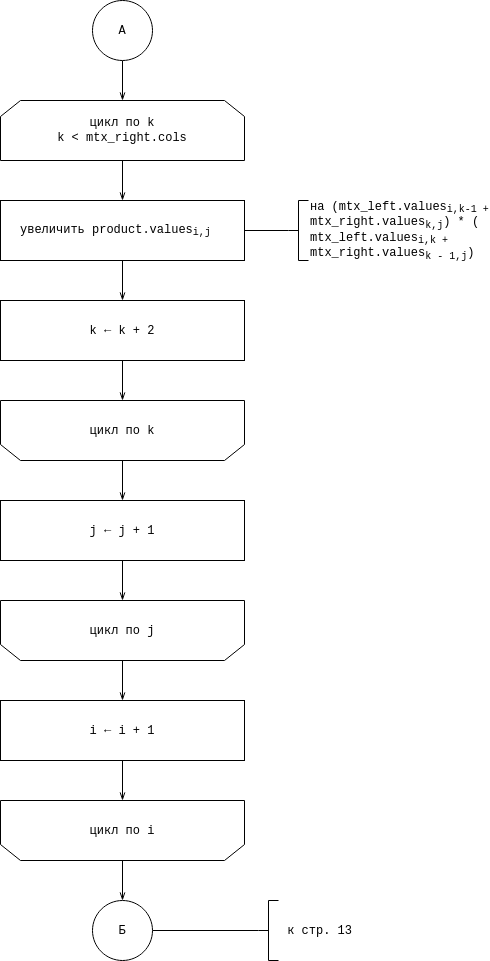
\includegraphics[width=0.7\linewidth]{assets/mtx-win2.drawio.png}
	\caption{Схема алгоритма умножения матриц Копперсмита -- Винограда (продолжение)}
	\label{fig:win-2}
\end{figure}

\begin{figure}[H]
	\centering
	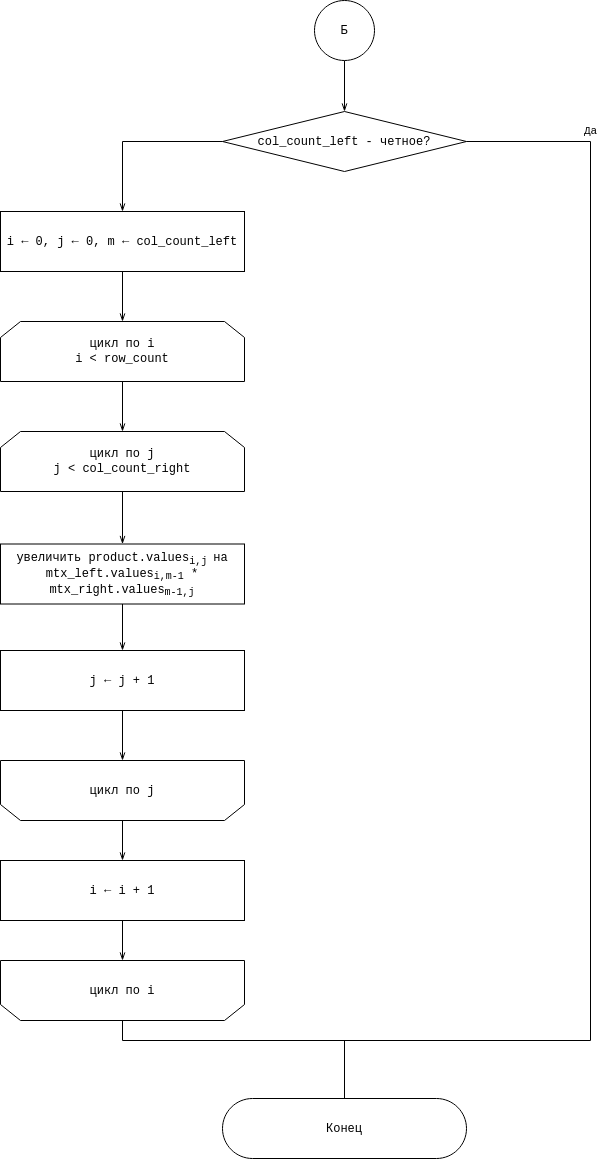
\includegraphics[width=0.7\linewidth]{assets/mtx-win3.drawio.png}
	\caption{Схема алгоритма умножения матриц Копперсмита -- Винограда (конец)}
	\label{fig:win-3}
\end{figure}

\begin{figure}[H]
	\centering
	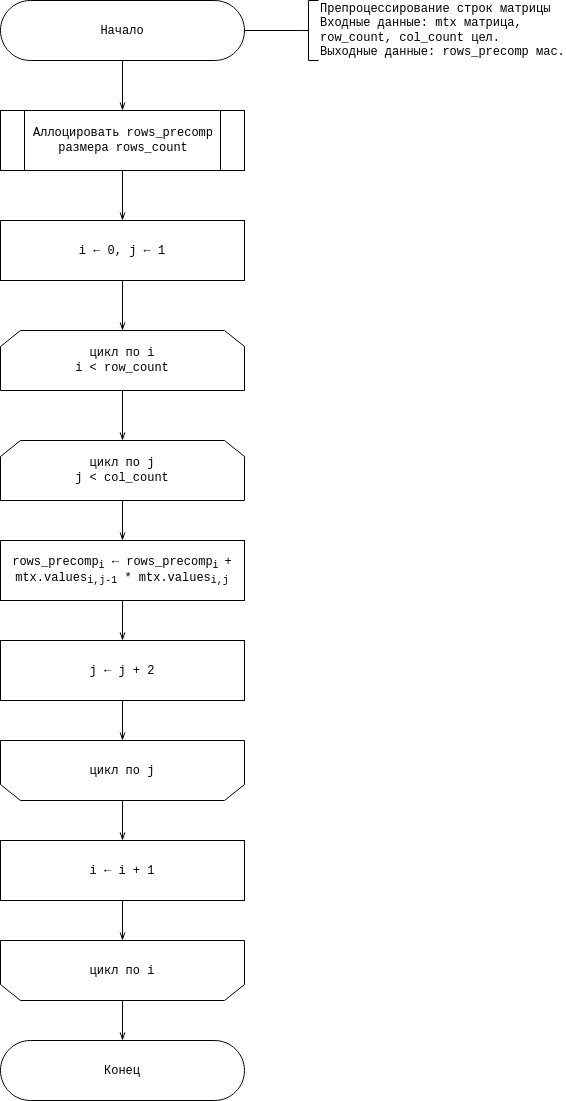
\includegraphics[width=0.7\linewidth]{assets/mtx-predproc-r.drawio.png}
	\caption{Алгоритм препроцессирования сторк}
	\label{fig:prep-r}
\end{figure}

\begin{figure}[H]
	\centering
	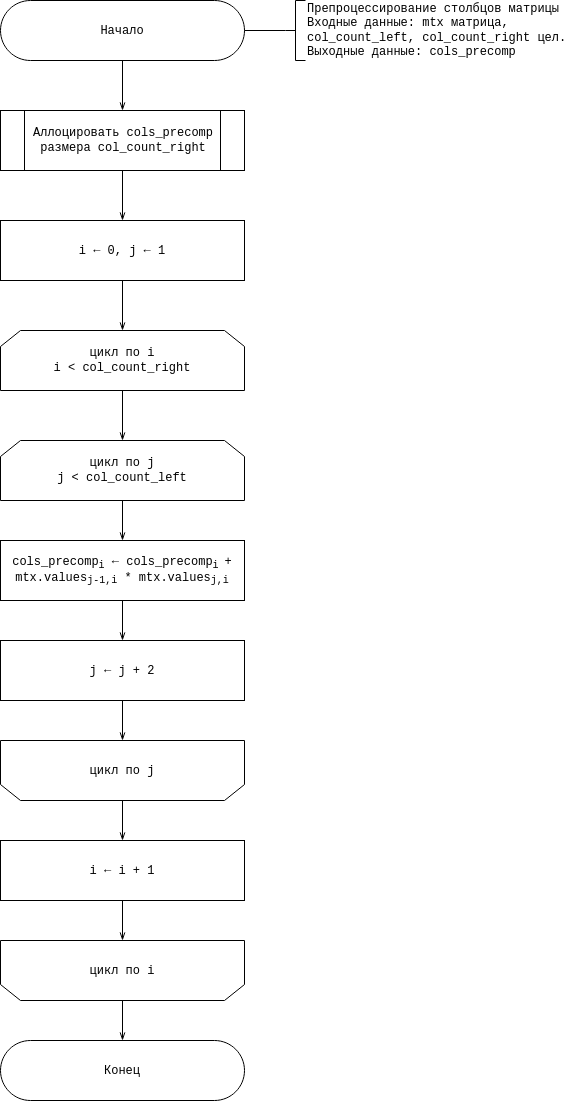
\includegraphics[width=0.7\linewidth]{assets/mtx-predproc-c.drawio.png}
	\caption{Схема алгоритма препроцессирования столбцов}
	\label{fig:prep-c}
\end{figure}

\begin{figure}[H]
	\centering
	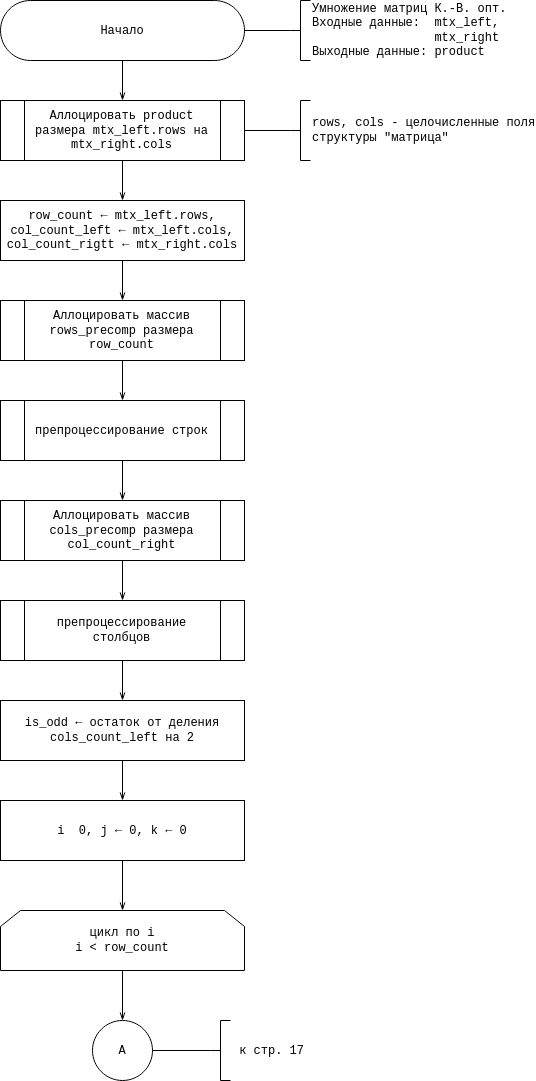
\includegraphics[width=0.7\linewidth]{assets/mtx-win-o-1.drawio.png}
	\caption{Схема оптимизированного алгоритма умножения матриц Копперсмита -- Винограда (начало)}
	\label{fig:win-o-1}
\end{figure}

\begin{figure}[H]
	\centering
	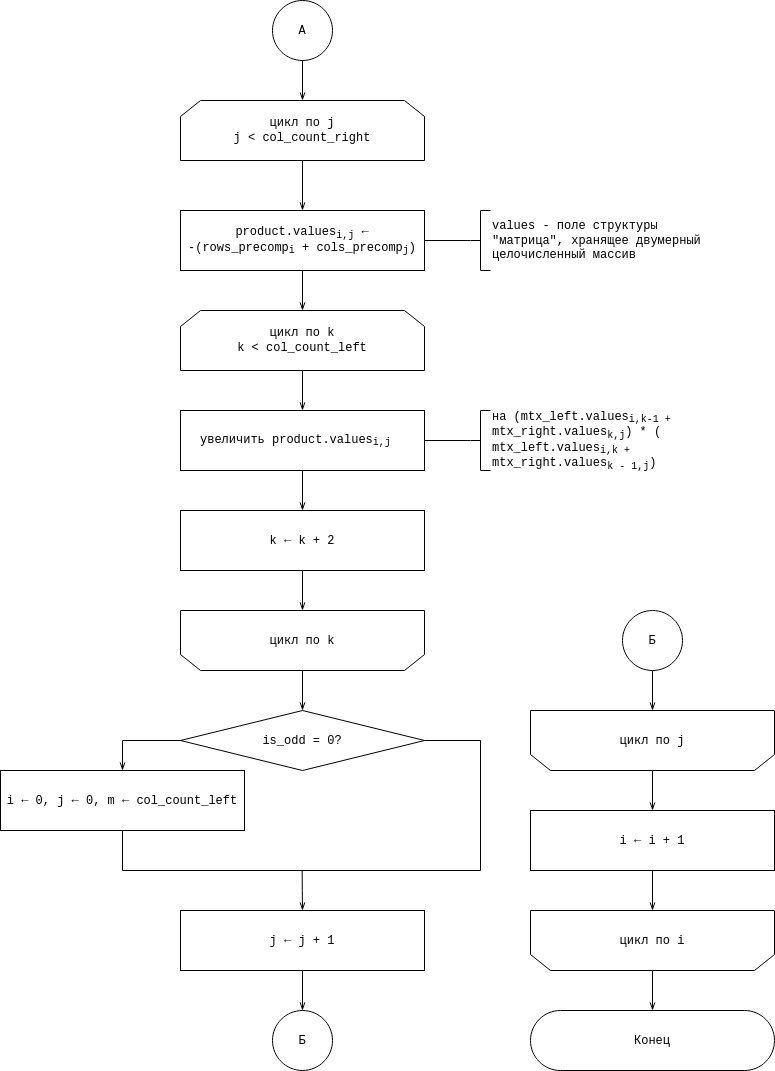
\includegraphics[width=0.9\linewidth]{assets/mtx-win-o-2.drawio.png}
	\caption{Схема оптимизированного алгоритма умножения матриц Копперсмита -- Винограда (конец)}
	\label{fig:win-o-2}
\end{figure}

\subsection{Вывод}
Алгоритмы были проанализированы с точки зрения временных затрат. Было выявлено, что алгоритм Копперсмита -- Винограда работает на \\ $0.5MNK$ быстрее, чем классический матричный. Оптимизация алгоритма же дает выигрыш на $1.5MNK$. 


Были построены схемы алгоритмов. Теоретически были исследованы способы оптимизации алгоритма Копперсмита -- Винограда. Было получено достаточно теоретических сведений для разработки ПО, решающего поставленную задачу.